% ============================================================
%  Ramanalyze / Modèle Excel : Guide de saisie terrain
%  Pour les préleveur·ses et bénévoles de terrain
% ============================================================

\documentclass[12pt, a4paper]{article}

% ── Encodage et langue ───────────────────────────────────────
\usepackage[utf8]{inputenc}
\usepackage[T1]{fontenc}
\usepackage[french]{babel}

% ── Mise en page ─────────────────────────────────────────────
\usepackage[top=2.5cm, bottom=2.8cm, left=2.8cm, right=2.8cm]{geometry}
\usepackage{parskip}
\usepackage{microtype}
\usepackage{lmodern}
\usepackage{setspace}
\setstretch{1.15}

% ── Couleurs ─────────────────────────────────────────────────
\usepackage{xcolor}
\definecolor{mainblue}{RGB}{25, 90, 160}
\definecolor{accentteal}{RGB}{20, 140, 130}
\definecolor{warnorange}{RGB}{210, 100, 20}
\definecolor{tipgreen}{RGB}{40, 140, 75}
\definecolor{stepbg}{RGB}{235, 242, 252}
\definecolor{figbg}{RGB}{225, 232, 240}
\definecolor{lightgray}{RGB}{245, 246, 248}
\definecolor{darkgray}{RGB}{80, 85, 95}
\definecolor{rulecolor}{RGB}{185, 195, 215}
\definecolor{tab1col}{RGB}{188, 224, 60}
\definecolor{tab5col}{RGB}{26, 122, 52}
\definecolor{xlsgreen}{RGB}{70, 160, 70}
\definecolor{xlsbg}{RGB}{232, 247, 232}
\definecolor{appblue}{RGB}{38, 50, 56}

% ── Graphique et TikZ ─────────────────────────────────────────
\usepackage{graphicx}
\usepackage{float}
\usepackage{tikz}
\usetikzlibrary{positioning, shapes.geometric, calc}

% ── Symboles ─────────────────────────────────────────────────
\usepackage{amssymb}
\usepackage{pifont}

% ── Tableaux ─────────────────────────────────────────────────
\usepackage{booktabs}
\usepackage{tabularx}
\usepackage{array}
\usepackage{longtable}
\newcolumntype{L}[1]{>{\raggedright\arraybackslash}p{#1}}
\newcolumntype{C}[1]{>{\centering\arraybackslash}p{#1}}

% ── Encadrés (tcolorbox) ─────────────────────────────────────
\usepackage{tcolorbox}
\tcbuselibrary{skins, breakable}

\newtcolorbox{conseil}{
  enhanced, breakable,
  colback=tipgreen!8!white, colframe=tipgreen!65!black,
  left=6pt, right=6pt, top=4pt, bottom=4pt,
  arc=4pt, boxrule=0.7pt,
  title={\small\bfseries Conseil},
  fonttitle=\small\bfseries,
  attach boxed title to top left={yshift=-2pt, xshift=6pt},
  boxed title style={colback=tipgreen!65!black, colframe=tipgreen!65!black,
                     arc=3pt, boxrule=0pt},
}

\newtcolorbox{attention}{
  enhanced, breakable,
  colback=warnorange!8!white, colframe=warnorange!75!black,
  left=6pt, right=6pt, top=4pt, bottom=4pt,
  arc=4pt, boxrule=0.7pt,
  title={\small\bfseries À noter},
  fonttitle=\small\bfseries,
  attach boxed title to top left={yshift=-2pt, xshift=6pt},
  boxed title style={colback=warnorange!75!black, colframe=warnorange!75!black,
                     arc=3pt, boxrule=0pt},
}

\newtcolorbox{enresume}{
  enhanced, breakable,
  colback=mainblue!6!white, colframe=mainblue!55!black,
  left=6pt, right=6pt, top=4pt, bottom=4pt,
  arc=4pt, boxrule=0.7pt,
  title={\small\bfseries En résumé},
  fonttitle=\small\bfseries,
  attach boxed title to top left={yshift=-2pt, xshift=6pt},
  boxed title style={colback=mainblue!55!black, colframe=mainblue!55!black,
                     arc=3pt, boxrule=0pt},
}

\newtcolorbox{methodebox}[1]{
  enhanced, breakable,
  colback=#1!6!white, colframe=#1!70!black,
  left=8pt, right=8pt, top=6pt, bottom=6pt,
  arc=5pt, boxrule=1pt,
}

% ── Listes ───────────────────────────────────────────────────
\usepackage{enumitem}
\setlist[enumerate]{itemsep=3pt, parsep=0pt, topsep=4pt}
\setlist[itemize]{itemsep=3pt, parsep=0pt, topsep=4pt}

% ── Titres de sections ────────────────────────────────────────
\usepackage[explicit]{titlesec}

\titleformat{\section}
  {\normalfont\large\bfseries\color{mainblue}}
  {\thesection}{0.7em}{#1}
  [\vspace{2pt}{\color{rulecolor}\rule{\linewidth}{0.8pt}}\vspace{2pt}]

\titleformat{\subsection}
  {\normalfont\normalsize\bfseries\color{accentteal}}
  {\thesubsection}{0.5em}{#1}

\titleformat{\subsubsection}
  {\normalfont\normalsize\bfseries\color{darkgray}}
  {\thesubsubsection}{0.5em}{#1}

\titlespacing*{\section}{0pt}{14pt}{6pt}
\titlespacing*{\subsection}{0pt}{10pt}{4pt}

% ── En-tête et pied de page ───────────────────────────────────
\usepackage{fancyhdr}
\pagestyle{fancy}
\fancyhf{}
\renewcommand{\headrulewidth}{0pt}
\fancyhead[L]{\small\color{darkgray}\textit{Ramanalyze : Guide saisie terrain}}
\fancyhead[R]{\small\color{darkgray}\thepage}
\fancyfoot[C]{\small\color{darkgray}\textit{CitizenSers : Usage interne}}

% ── Hyperliens ────────────────────────────────────────────────
\usepackage[hidelinks, colorlinks=true,
            linkcolor=mainblue, urlcolor=accentteal]{hyperref}

% ──────────────────────────────────────────────────────────────
%  Commandes personnalisées
% ──────────────────────────────────────────────────────────────

\newcommand{\numcercle}[1]{%
  \tikz[baseline=(n.base)]{%
    \node[circle, fill=mainblue, text=white,
          inner sep=2.5pt, font=\bfseries\small] (n) {#1};}%
}

\newcommand{\etape}[2]{%
  \vspace{10pt}%
  \noindent\numcercle{#1}\enskip
  {\large\bfseries\color{mainblue}#2}\par
  \vspace{3pt}%
  \noindent{\color{rulecolor}\rule{\linewidth}{0.4pt}}\par
  \vspace{4pt}%
}

\newcommand{\bouton}[1]{%
  \tikz[baseline=(b.base)]{%
    \node[rounded corners=3pt, fill=darkgray!12, draw=darkgray!35,
          inner xsep=5pt, inner ysep=2pt,
          font=\small\bfseries\color{darkgray}] (b) {#1};}%
}

\newcommand{\onglet}[1]{\textbf{\color{mainblue}#1}}
\newcommand{\champ}[1]{\textit{\color{accentteal}\og\,#1\,\fg{}}}
\newcommand{\cellule}[1]{\texttt{\color{mainblue}#1}}

% Badge "Logiciel" ou "Excel"
\newcommand{\badgelogiciel}{%
  \tikz[baseline=(b.base)]{%
    \node[rounded corners=3pt, fill=appblue, draw=appblue!70!black,
          inner xsep=5pt, inner ysep=2pt,
          font=\small\bfseries\color{white}] (b) {Logiciel};}%
}
\newcommand{\badgeexcel}{%
  \tikz[baseline=(b.base)]{%
    \node[rounded corners=3pt, fill=xlsgreen, draw=xlsgreen!70!black,
          inner xsep=5pt, inner ysep=2pt,
          font=\small\bfseries\color{white}] (b) {Excel};}%
}

% Placeholder de capture d'écran
\newcommand{\figph}[2][Capture d'écran]{%
  \begin{figure}[H]
    \centering
    \begin{tikzpicture}
      \node[
        draw=rulecolor, fill=figbg, rounded corners=5pt,
        minimum width=0.92\linewidth, minimum height=4.2cm,
        align=center, text width=0.82\linewidth,
        font=\small\color{darkgray}
      ] {%
        {\large\bfseries\color{rulecolor!70!darkgray}%
         \MakeUppercase{[ capture d'écran ]}}\\[8pt]#2%
      };
    \end{tikzpicture}
    \caption{#1}
  \end{figure}%
}

% ──────────────────────────────────────────────────────────────
\begin{document}

% ── Page de titre ─────────────────────────────────────────────
\begin{titlepage}
  \centering
  \vspace*{1.2cm}

  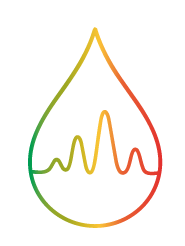
\includegraphics[width=0.28\linewidth]{../../Logo Ramanalyze/logo ramanalyze.pdf}

  \vspace{1.4cm}

  {\Huge\bfseries\color{tab5col} Ramanalyze}\\[8pt]
  {\large\color{darkgray} Guide de saisie terrain}

  \vspace{0.8cm}
  {\large\color{darkgray}
    Comment renseigner les informations de prélèvement\\
    dans le logiciel ou dans le fichier Excel.}

  \vspace{0.5cm}
  {\normalsize\color{darkgray}
    À destination des préleveur·ses et bénévoles de terrain.\\
    Aucune connaissance technique préalable requise.}

  \vspace{2cm}

  % Schéma des deux méthodes
  \begin{tikzpicture}
    \node[rounded corners=6pt, fill=appblue, draw=appblue!70!black,
          minimum width=5.5cm, minimum height=1.4cm,
          align=center, font=\bfseries\color{white}]
         (soft) {\Large Logiciel\\[-2pt]\small Ramanalyze};
    \node[right=2.2cm of soft,
          rounded corners=6pt, fill=xlsgreen, draw=xlsgreen!70!black,
          minimum width=5.5cm, minimum height=1.4cm,
          align=center, font=\bfseries\color{white}]
         (xls) {\Large Fichier Excel\\[-2pt]\small modèle final.xlsx};
    \node[above=0.7cm of soft, xshift=3.85cm,
          font=\large\bfseries\color{darkgray}] (ou) {OU};
    \draw[dashed, thick, color=darkgray!50] (soft.east) -- (xls.west);
  \end{tikzpicture}

  \vspace{1.8cm}

  \begin{tcolorbox}[
    enhanced, colback=mainblue!5!white, colframe=mainblue!50!black,
    width=0.82\linewidth, arc=5pt, boxrule=0.8pt,
    left=10pt, right=10pt, top=8pt, bottom=8pt
  ]
    \centering
    Ce document explique \textbf{champ par champ} ce qu'il faut
    renseigner lors d'un prélèvement, quelle que soit la méthode choisie.
  \end{tcolorbox}

  \vfill

  {\color{darkgray}\small
    \textbf{CitizenSers} : Document à usage interne\\[6pt]
    Pour toute question, contactez la personne responsable du suivi.
  }
\end{titlepage}

\newpage
\tableofcontents
\newpage

% ══════════════════════════════════════════════════════════════
\section{Avant de commencer}
% ══════════════════════════════════════════════════════════════

\subsection{À quoi servent ces informations ?}

Chaque prélèvement doit être accompagné d'une fiche de terrain
regroupant toutes les informations contextuelles : qui a prélevé,
où, quand, dans quelles conditions, et quelles mesures ont été
réalisées sur place.

Ces informations permettent ensuite :
\begin{itemize}
  \item d'identifier sans ambiguïté chaque échantillon ;
  \item de relier les spectres Raman à l'échantillon correspondant ;
  \item d'analyser les résultats en tenant compte du contexte
        (météo, type d'eau, heure de marée, etc.).
\end{itemize}

\begin{attention}
  Une fiche incomplète ou incorrecte peut rendre un échantillon
  inutilisable. Prenez le temps de remplir chaque champ avec soin,
  même si certaines informations vous semblent secondaires.
\end{attention}

\subsection{Deux méthodes au choix}

\begin{center}
\begin{tabularx}{0.88\linewidth}{C{0.38\linewidth} C{0.06\linewidth} C{0.38\linewidth}}
  \toprule
  \textbf{Logiciel Ramanalyze} & \textbf{OU} & \textbf{Fichier Excel} \\
  \textit{modèle final.xlsx} & & \\
  \midrule
  Interface graphique guidée & & Fichier Excel autonome \\
  Nom généré automatiquement & & À remplir cellule par cellule \\
  Export structuré \texttt{.xlsx} & & Export direct du fichier \\
  Recommandé si vous avez accès & & Utilisable sans le logiciel \\
  au logiciel & & installé \\
  \bottomrule
\end{tabularx}
\end{center}

Les deux méthodes produisent exactement les mêmes informations.
Le logiciel peut ensuite charger un fichier Excel rempli à la main.

\subsection{Le nom du prélèvement}

Le \textbf{nom du prélèvement} est l'identifiant central de toute
la session. Il suit le format :

\begin{center}
  \large\texttt{PRE\_<initiales>\_AAAAMMJJ\_HHhMM}
\end{center}

\begin{itemize}
  \item \texttt{PRE\_} : préfixe fixe, toujours présent.
  \item \texttt{<initiales>} : 1\textsuperscript{re} lettre du prénom + 1\textsuperscript{re}
        lettre du nom de \emph{chaque} préleveur·se, concaténées.\\
        Exemple : Denis Jacquet et Alice Martin → \texttt{DJAM}
  \item \texttt{AAAAMMJJ} : date au format année-mois-jour.
  \item \texttt{HHhMM} : heure et minutes du prélèvement.
\end{itemize}

\begin{center}
  \large\textbf{Exemple complet :} \texttt{PRE\_DJAM\_20260504\_10h30}
\end{center}

\begin{conseil}
  Traitez ce nom comme le \textbf{code-barres} de votre échantillon :
  il doit être unique et ne jamais être réutilisé pour un autre prélèvement.
  Dans le logiciel, il est généré automatiquement dès que les
  préleveur·ses et la date/heure sont renseignés.
\end{conseil}

\newpage

% ══════════════════════════════════════════════════════════════
\section{Méthode 1 — Logiciel Ramanalyze}
% ══════════════════════════════════════════════════════════════

Ouvrez le logiciel et cliquez sur l'onglet \onglet{Métadonnées}.

\figph[Onglet Métadonnées ouvert — vue générale]{%
  L'onglet Métadonnées avec toutes les sections visibles :\\
  préleveur·ses, localisation, contexte terrain, mesures.}

\subsection{Charger une fiche existante (optionnel)}

Si une fiche a déjà été partiellement enregistrée, cliquez sur
\bouton{Charger des métadonnées\ldots} en haut de l'onglet pour
la reprendre. Sinon, continuez directement avec une fiche vierge.

% ─────────────────────────────────────────────────────────────
\subsection{Section 1 : Identification du prélèvement}
% ─────────────────────────────────────────────────────────────

\etape{1}{Renseigner les préleveur·ses}

\begin{itemize}
  \item Saisissez \textbf{Prénom puis nom} dans le champ
        \champ{Préleveur·se} (ex. : \texttt{Denis Jacquet}).
  \item Indiquez l'association correspondante dans le champ
        \champ{Association}.
  \item S'il y a plusieurs préleveur·ses, cliquez sur
        \bouton{+1 préleveur·se} pour ajouter une ligne.
\end{itemize}

\begin{conseil}
  Le format \textbf{Prénom Nom} est important : le logiciel extrait
  les initiales pour générer automatiquement le nom du prélèvement.
\end{conseil}

\etape{2}{Renseigner la date et l'heure}

Cliquez sur les champs \champ{Date du prélèvement} et
\champ{Heure du prélèvement} et saisissez les valeurs correspondantes.
Ces champs passent au vert une fois renseignés.

Le \textbf{nom du prélèvement} \texttt{PRE\_\ldots} s'affiche alors
automatiquement dans le champ en dessous.

\etape{3}{Vérifier le nom du prélèvement}

Le champ \champ{Nom du prélèvement} est généré automatiquement.
Vérifiez qu'il correspond bien à votre session.
Si besoin, il peut être modifié à la main.

% ─────────────────────────────────────────────────────────────
\subsection{Section 2 : Localisation}
% ─────────────────────────────────────────────────────────────

\etape{4}{Type de lieu et nom du point}

\begin{itemize}
  \item \champ{Type de lieu} : choisissez dans la liste déroulante
        le type qui correspond le mieux au site de prélèvement
        (plage, cours d'eau, estuaire, etc.).
  \item \champ{Nom du point de prélèvement} : saisissez le nom
        local du site (ex. : \texttt{Plage du Bon Secours}).
\end{itemize}

\etape{5}{Coordonnées GPS}

\begin{itemize}
  \item Saisissez la \champ{Latitude} et la \champ{Longitude} en
        degrés décimaux (ex. : \texttt{48.639} et \texttt{-2.022}).
  \item Les coordonnées issues d'une application GPS ou d'un
        téléphone sont acceptées directement.
  \item Le bouton \bouton{Carte / pointer\ldots} ouvre une carte
        interactive pour placer le point à la souris.
\end{itemize}

\begin{conseil}
  Si la connexion Internet est disponible, le \textbf{département}
  et la \textbf{commune} se remplissent automatiquement après
  la saisie des coordonnées GPS. Vérifiez et corrigez si besoin.
\end{conseil}

\etape{6}{Département et commune}

Si les champs \champ{Département} et \champ{Commune} ne se sont
pas remplis automatiquement, saisissez-les manuellement.

% ─────────────────────────────────────────────────────────────
\subsection{Section 3 : Contexte terrain}
% ─────────────────────────────────────────────────────────────

\etape{7}{Type d'eau}

Sélectionnez le \champ{Type d'eau} dans la liste déroulante.
Ce champ reste en rouge tant qu'aucun choix n'est fait.

\begin{itemize}
  \item \textbf{Eau de mer} ou \textbf{eau estuarienne} : des champs
        supplémentaires apparaissent pour le \champ{Coefficient de marée}
        et l'\champ{Heure de pleine mer}.
  \item \textbf{Eau douce} : le bouton \bouton{Débit / flux\ldots}
        devient disponible pour saisir largeur, hauteur d'eau, vitesse
        et débit si la mesure a été réalisée.
\end{itemize}

\etape{8}{Conditions météo et températures}

Renseignez les champs disponibles en fonction de ce qui a été mesuré :

\begin{center}
\begin{tabularx}{0.9\linewidth}{L{4.8cm} L{7cm}}
  \toprule
  \textbf{Champ} & \textbf{Ce qu'il faut saisir} \\
  \midrule
  Temps au moment de la mesure & Météo générale (liste déroulante) \\
  Température de l'eau & En °C, mesurée sur site \\
  Température de l'air & En °C \\
  Pluie dernières 24 h & En mm (si connue) \\
  \bottomrule
\end{tabularx}
\end{center}

% ─────────────────────────────────────────────────────────────
\subsection{Section 4 : Mesures terrain}
% ─────────────────────────────────────────────────────────────

Cochez uniquement les mesures qui ont été réalisées sur place.
Chaque case cochée affiche les champs correspondants.

\etape{9}{Test ammonium}

Si un test ammonium a été réalisé, cochez \champ{Test ammonium réalisé}.
Renseignez :
\begin{itemize}
  \item \champ{Réalisé par} : prénom + nom de la personne qui a fait le test.
  \item \champ{Test 1 (grossier)} : résultat du premier test colorimétrique.
  \item \champ{Test 2 (précis)} : résultat du second test si réalisé.
  \item \champ{pH (ammonium)} : valeur du pH mesurée lors du test.
\end{itemize}

\begin{conseil}
  Si vous renseignez le \champ{pH (ammonium)}, le champ
  \champ{pH de l'eau} (mesures terrain) se remplit automatiquement
  avec la même valeur.
\end{conseil}

\etape{10}{Analyses bactériologiques}

Si des prélèvements pour analyses bactériologiques ont été effectués,
cochez \champ{Analyses bactériologiques}. Renseignez :
\begin{itemize}
  \item \champ{Jour de dépôt} et \champ{Heure de dépôt} : quand les
        flacons seront déposés au laboratoire.
  \item \champ{Entreprise de mesure} : nom du laboratoire.
  \item \champ{Résultats E. coli} et \champ{Résultats Entérocoques} :
        à compléter ultérieurement si les résultats arrivent après.
\end{itemize}

\etape{11}{Autres mesures terrain}

Cochez les mesures effectuées et saisissez la valeur correspondante :

\begin{center}
\begin{tabularx}{0.9\linewidth}{L{4.2cm} L{2.2cm} L{5.5cm}}
  \toprule
  \textbf{Mesure} & \textbf{Unité} & \textbf{Remarque} \\
  \midrule
  Turbidité & NTU & Mesurée avec un turbidimètre \\
  Conductivité & µS/cm & Mesurée avec un conductimètre \\
  pH de l'eau & --- & 0 à 14 \\
  Oxygène dissous & mg/L & Mesurée avec un oxymètre \\
  \bottomrule
\end{tabularx}
\end{center}

% ─────────────────────────────────────────────────────────────
\subsection{Enregistrer la fiche}
% ─────────────────────────────────────────────────────────────

\etape{12}{Enregistrer le fichier Excel}

Cliquez sur \bouton{Enregistrer les métadonnées\ldots} en bas de
l'onglet. Le logiciel propose un nom de fichier basé sur le nom du
prélèvement. Validez ou choisissez un autre emplacement.

Le fichier \texttt{.xlsx} créé contient plusieurs feuilles :

\begin{center}
\begin{tabularx}{0.88\linewidth}{L{4.5cm} L{7.5cm}}
  \toprule
  \textbf{Feuille} & \textbf{Contenu} \\
  \midrule
  \texttt{Mesures} & Fiche terrain synthétique, lisible directement \\
  \texttt{Index-métadonnées} & Données techniques pour rechargement \\
  \texttt{Titration-\ldots} & Volumes et correspondance (si titration) \\
  \bottomrule
\end{tabularx}
\end{center}

Le nom de fichier suit la convention :
\texttt{PRE\_DJAM\_20260504\_10h30\_T\_AnBa\_TAm.xlsx}
avec les suffixes optionnels :

\begin{center}
\begin{tabularx}{0.72\linewidth}{C{1.6cm} L{8cm}}
  \toprule
  \textbf{Suffixe} & \textbf{Signification} \\
  \midrule
  \texttt{\_T} & Titration du cuivre prévue \\
  \texttt{\_AnBa} & Analyses bactériologiques \\
  \texttt{\_TAm} & Test ammonium réalisé \\
  \texttt{\_Tur} & Turbidité mesurée \\
  \texttt{\_Cond} & Conductivité mesurée \\
  \texttt{\_pH} & pH de l'eau mesuré \\
  \texttt{\_Ox} & Oxygène dissous mesuré \\
  \bottomrule
\end{tabularx}
\end{center}

\newpage

% ══════════════════════════════════════════════════════════════
\section{Méthode 2 — Fichier Excel \texttt{modèle final.xlsx}}
% ══════════════════════════════════════════════════════════════

Cette méthode est à utiliser si le logiciel n'est pas disponible ou
si vous préférez travailler directement dans Excel.

Ouvrez le fichier \texttt{modèle final.xlsx}. Il contient une seule
feuille nommée \textbf{Mesures}.

\figph[Feuille Mesures du fichier Excel modèle]{%
  Structure de la feuille Mesures : bloc d'identification en haut,\\
  sections de mesures terrain en dessous.}

\subsection{Bloc d'identification (lignes 1 à 7)}

\begin{center}
\begin{tabularx}{0.92\linewidth}{C{1.2cm} C{1.5cm} L{4cm} L{6.2cm}}
  \toprule
  \textbf{Ligne} & \textbf{Colonne} & \textbf{Champ} & \textbf{Ce qu'il faut saisir} \\
  \midrule
  3 & B & Nom du prélèvement & Identifiant unique, format \texttt{PRE\_...} \\
  3 & D & Type d'eau & Eau douce / mer / estuarienne \\
  4 & B & Département & Numéro ou nom du département \\
  4 & D & Commune & Nom de la commune \\
  5 & B & Date du prélèvement & Format \texttt{JJ/MM/AAAA} \\
  5 & D & Heure du prélèvement & Format \texttt{HH:MM} \\
  6 & B & Type de lieu & Plage, cours d'eau, estuaire\ldots \\
  6 & D & Nom du point & Nom local du site de prélèvement \\
  7 & B & Latitude & Degrés décimaux (ex. : 48.639) \\
  7 & D & Longitude & Degrés décimaux (ex. : -2.022) \\
  \bottomrule
\end{tabularx}
\end{center}

\subsection{Bloc préleveur·ses (lignes 8 et suivantes)}

Chaque ligne correspond à un·e préleveur·se :

\begin{center}
\begin{tabularx}{0.72\linewidth}{C{1.5cm} C{1.5cm} L{8.5cm}}
  \toprule
  \textbf{Colonne} & & \textbf{Ce qu'il faut saisir} \\
  \midrule
  A & (label) & \texttt{Préleveur·se 1}, \texttt{Préleveur·se 2}\ldots \\
  B & & Prénom + Nom de la personne \\
  C & (label) & \texttt{Association} \\
  D & & Nom de l'association \\
  \bottomrule
\end{tabularx}
\end{center}

\begin{conseil}
  S'il y a plusieurs préleveur·ses, ajoutez des lignes en copiant
  le format de la ligne 8 (labels en A et C, valeurs en B et D).
\end{conseil}

\subsection{Cases à cocher — statut des mesures}

Les deux lignes suivant les préleveur·ses indiquent quelles mesures
ont été réalisées. Remplacez \texttt{Non} par \texttt{Oui} pour chaque
mesure effectuée :

\begin{center}
\begin{tabularx}{0.82\linewidth}{L{5.5cm} C{2cm} L{4cm}}
  \toprule
  \textbf{Champ} & \textbf{Valeur} & \textbf{Colonne} \\
  \midrule
  Titration du cuivre & Oui / Non & A \\
  Analyses bactériologiques & Oui / Non & C \\
  Test ammonium réalisé & Oui / Non & E \\
  Turbidité mesurée & Oui / Non & G \\
  Conductivité mesurée & Oui / Non & A (ligne suivante) \\
  pH eau mesuré & Oui / Non & C \\
  Oxygène dissous mesuré & Oui / Non & E \\
  \bottomrule
\end{tabularx}
\end{center}

\subsection{Sections de mesures}

Les sections suivantes (contexte terrain, test ammonium, bactériologie,
autres mesures, titration) contiennent chacune une ligne de labels
et une ligne de valeurs.

\begin{center}
\begin{longtable}{L{4.8cm} L{2.8cm} L{5.5cm}}
  \toprule
  \textbf{Champ} & \textbf{Unité} & \textbf{Remarque} \\
  \midrule
  \endhead
  \multicolumn{3}{l}{\textit{Contexte terrain}} \\
  \midrule
  Temps au moment de la mesure & --- & Ensoleillé, nuageux, pluvieux\ldots \\
  Température de l'eau & °C & \\
  Température de l'air & °C & \\
  Pluie dernières 24 h & mm & \\
  Coefficient de marée & --- & Eau de mer / estuarienne uniquement \\
  Heure de pleine mer & HH:MM & Eau de mer / estuarienne uniquement \\
  \midrule
  \multicolumn{3}{l}{\textit{Test ammonium}} \\
  \midrule
  Test ammonium réalisé & Oui/Non & Reprend la valeur du bloc statut \\
  Test ammonium réalisé par & --- & Prénom + Nom \\
  Test ammonium 1 (grossier) & --- & Résultat colorimétrique \\
  Test ammonium 2 (précis) & --- & Résultat colorimétrique \\
  pH (ammonium) & --- & Valeur mesurée \\
  \midrule
  \multicolumn{3}{l}{\textit{Analyses bactériologiques}} \\
  \midrule
  Analyses bactériologiques & Oui/Non & Reprend la valeur du bloc statut \\
  Jour de dépôt & JJ/MM/AAAA & \\
  Heure du dépôt & HH:MM & \\
  Entreprise de mesure & --- & Nom du laboratoire \\
  Résultats E. coli & npp/ml & À compléter après réception \\
  Résultats Entérocoques & npp/100ml & À compléter après réception \\
  \midrule
  \multicolumn{3}{l}{\textit{Autres mesures terrain}} \\
  \midrule
  Turbidité mesurée & Oui/Non & \\
  Turbidité & NTU & \\
  Conductivité mesurée & Oui/Non & \\
  Conductivité & µS/cm & \\
  pH de l'eau mesuré & Oui/Non & \\
  pH de l'eau & --- & \\
  Oxygène dissous mesuré & Oui/Non & \\
  Oxygène dissous & mg/L & \\
  \midrule
  \multicolumn{3}{l}{\textit{Titration du cuivre}} \\
  \midrule
  Titration du cuivre & Oui/Non & \\
  Nom de la manip de titration & --- & Format \texttt{INITIALES\_AAAAMMJJ\_HHhMM} \\
  Date de la titration & JJ/MM/AAAA & \\
  Heure de la titration & HH:MM & \\
  Lieu de la titration & --- & \\
  \midrule
  \multicolumn{3}{l}{\textit{Commentaires}} \\
  \midrule
  Commentaire sur les conditions & --- & Texte libre \\
  \bottomrule
\end{longtable}
\end{center}

\begin{attention}
  Le fichier Excel ne génère pas automatiquement le nom du prélèvement.
  Saisissez-le manuellement en ligne 3, colonne B, en respectant le
  format \texttt{PRE\_<initiales>\_AAAAMMJJ\_HHhMM}.
\end{attention}

\newpage

% ══════════════════════════════════════════════════════════════
\section{Récapitulatif et checklist}
% ══════════════════════════════════════════════════════════════

\subsection{Checklist de saisie terrain}

Avant de remettre ou d'enregistrer votre fiche, vérifiez que
chaque point est coché :

\begin{center}
\begin{tabularx}{0.88\linewidth}{C{0.8cm} L{10.5cm}}
  \toprule
  \textbf{} & \textbf{Point à vérifier} \\
  \midrule
  $\Box$ & Nom du prélèvement renseigné au format \texttt{PRE\_...} \\
  $\Box$ & Prénom et nom de chaque préleveur·se saisis \\
  $\Box$ & Association renseignée pour chaque préleveur·se \\
  $\Box$ & Date et heure du prélèvement renseignées \\
  $\Box$ & Coordonnées GPS saisies (latitude et longitude) \\
  $\Box$ & Type de lieu et nom du point renseignés \\
  $\Box$ & Département et commune renseignés \\
  $\Box$ & Type d'eau sélectionné \\
  $\Box$ & Conditions météo et températures notées \\
  $\Box$ & Mesures terrain cochées et valeurs saisies \\
  $\Box$ & Tests ammonium renseignés (si réalisés) \\
  $\Box$ & Bactériologie renseignée (si réalisée) \\
  $\Box$ & Fichier enregistré (logiciel) ou complété (Excel) \\
  \bottomrule
\end{tabularx}
\end{center}

\subsection{En cas de doute}

\begin{enresume}
  \begin{itemize}
    \item Si un champ n'est pas applicable (ex. coefficient de marée
          pour de l'eau douce), laissez-le vide.
    \item Si une valeur est incertaine, notez-la avec une mention
          dans les commentaires.
    \item En cas de question sur le format ou la procédure, contactez
          la personne responsable du suivi CitizenSers.
  \end{itemize}
\end{enresume}

\end{document}
